\documentclass[tikz,border=3pt]{standalone}
\usepackage{amsmath,amssymb}
\usepackage{sourcesanspro}
\usetikzlibrary{arrows.meta, positioning, calc}

\definecolor{cPrimal}{RGB}{0, 102, 180}
\definecolor{cDual}{RGB}{209, 34, 57}

\begin{document}
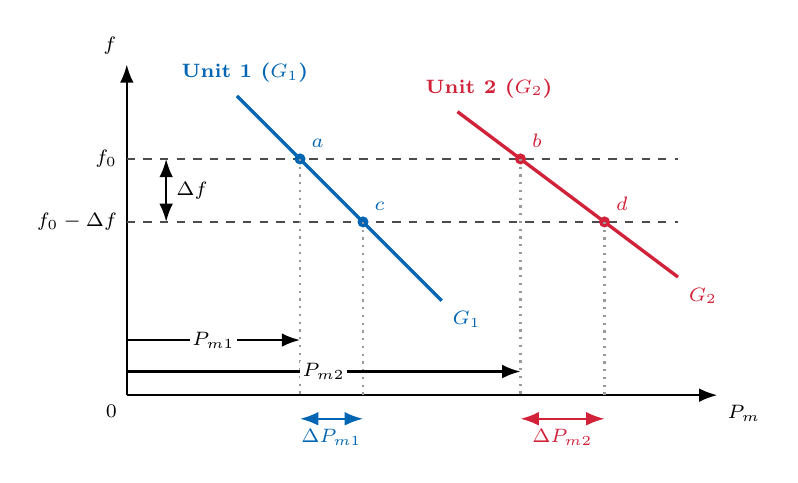
\begin{tikzpicture}[>=Latex, font=\scriptsize]
    % Coordinates:
    % f0 = 3.0, f_drop = 2.2 -> Delta f = 0.8
    % G1 (Unit 1): slope = -1.0
    %   point a at (2.2, 3.0) -> f0
    %   point c at (3.0, 2.2) -> f0 - Delta f
    %   Delta P_m1 = 0.8
    % G2 (Unit 2): slope = -0.75
    %   point b at (5.0, 3.0) -> f0
    %   point d at (6.067, 2.2) -> f0 - Delta f (Delta P_m2 = 1.067)
    
    % Axes
    \draw[->, thick] (0, 0) -- (7.5, 0) node[below right] {$P_m$};
    \draw[->, thick] (0, 0) -- (0, 4.2) node[above left] {$f$};
    \node[below left] at (0, 0) {$0$};

    % Frequency levels
    \draw[dashed, thick, black!70] (0, 3.0) -- (7.0, 3.0);
    \node[left] at (0, 3.0) {$f_0$};

    \draw[dashed, thick, black!70] (0, 2.2) -- (7.0, 2.2);
    \node[left] at (0, 2.2) {$f_0 - \Delta f$};

    % Delta f arrow
    \draw[<->, thick] (0.5, 3.0) -- (0.5, 2.2) node[midway, right] {$\Delta f$};

    % Unit 1 Droop Line (G1) - Blue
    \draw[very thick, cPrimal] (1.4, 3.8) -- (4.0, 1.2) node[below right] {$G_1$};
    \node[above, cPrimal, font=\bfseries\scriptsize] at (1.5, 3.85) {Unit 1 ($G_1$)};

    % Points a and c
    \fill[cPrimal] (2.2, 3.0) circle (2pt) node[above right=1pt] {$a$};
    \fill[cPrimal] (3.0, 2.2) circle (2pt) node[above right=1pt] {$c$};

    % Unit 2 Droop Line (G2) - Red
    \draw[very thick, cDual] (4.2, 3.6) -- (7.0, 1.5) node[below right] {$G_2$};
    \node[above, cDual, font=\bfseries\scriptsize] at (4.6, 3.65) {Unit 2 ($G_2$)};

    % Points b and d
    \fill[cDual] (5.0, 3.0) circle (2pt) node[above right=1pt] {$b$};
    \fill[cDual] (6.067, 2.2) circle (2pt) node[above right=1pt] {$d$};

    % Vertical drop lines
    \draw[dotted, thick, gray!80] (2.2, 3.0) -- (2.2, 0);
    \draw[dotted, thick, gray!80] (3.0, 2.2) -- (3.0, 0);
    \draw[dotted, thick, gray!80] (5.0, 3.0) -- (5.0, 0);
    \draw[dotted, thick, gray!80] (6.067, 2.2) -- (6.067, 0);

    % Power baseline arrows
    \draw[->, thick] (0, 0.7) -- (2.2, 0.7) node[midway, fill=white, inner sep=1pt] {$P_{m1}$};
    \draw[->, thick] (0, 0.3) -- (5.0, 0.3) node[midway, fill=white, inner sep=1pt] {$P_{m2}$};

    % Power increase arrows below axis
    \draw[<->, thick, cPrimal] (2.2, -0.3) -- (3.0, -0.3) node[midway, below] {$\Delta P_{m1}$};
    \draw[<->, thick, cDual] (5.0, -0.3) -- (6.067, -0.3) node[midway, below] {$\Delta P_{m2}$};
\end{tikzpicture}
\end{document}
